\section{Gestione della concorrenza}

\subsection{Concetti di base}
Per i SO moderni, é essenziale supportare piú processi in esecuzione:
\begin{itemize}
    \item \textbf{multiprogrammazione}: multiplo processi in memoria
    \item \textbf{multiprocessing}: multiplo processi in esecuzione
    \item \textbf{computazione distribuita}: multiplo processi in esecuzione su piú macchine
\end{itemize}
uno dei problemi principali é la \textbf{concorrenza}, ovvero gestire il modo con cui questi processi interagiscono tra di loro.
\begin{figure}
    \centering
    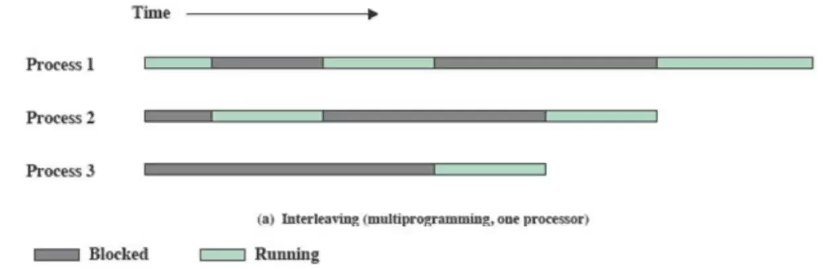
\includegraphics[width=0.5\linewidth]{immagini/multiprogrammazzione}
    \caption{Multiprogrammazione: un solo processore, piú processi in memoria}
\end{figure}
\begin{figure}
    \centering
    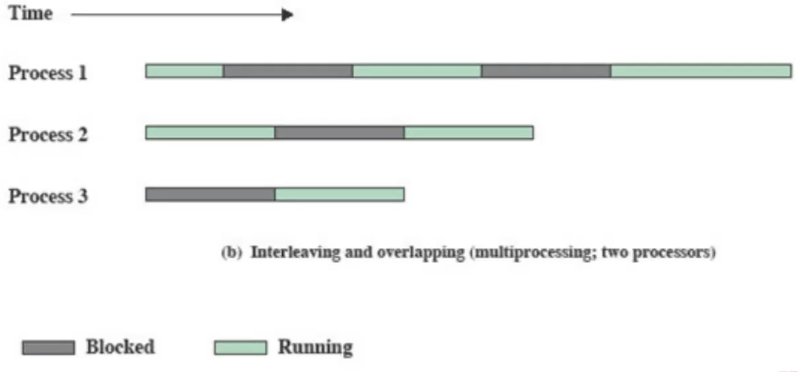
\includegraphics[width=0.5\linewidth]{immagini/MultiProcessing}
    \caption{Multiprocessing: piú processori, piú processi in esecuzione}
\end{figure}
Il problema della concorrenza si presenta in entrambi i casi, puuó succedere che ci siano applicazione diverse che sono in
esecuzione contemporaneamente, ci sono applicazioni che sono fatte per essere eseguite in parallelo, il sistema operativo stesso
puó avere piú processi in esecuzione, in tutti questi casi é necessario gestire la concorrenza.
\subsubsection*{Temini chiave}
\begin{itemize}
    \item \textbf{Mutua esclusione}: Ci sono 2 o piú processi che vogliono accedere alla stessa risorsa, peró solo uno alla volta puó accedere.
    \item \textbf{Sezione critica}: Parte del codice di un processo in cui viene effettuato un accesso a una risorsa condivisa.
    \item \textbf{Corsa critica(race condition)}: É un caso in cui la mutua esclusione non é rispettata, due o piú processi accedono alla stessa risorsa contemporaneamente.
    \item \textbf{Operazione Atomica}: É una sequenza indivisibile di comandi, nessun altro processo pu;o vedere uno stato intermedio della sequenza o interrompere la sequenza, durante una operazione atomica il dispatcher non puó intervenire.
    \item \textbf{Stallo (Deadlock)}: Situazione in cui due o piú processi sono in attesa di una risorsa che é posseduta da un altro processo, che a sua volta é in attesa di una risorsa posseduta da uno dei processi in attesa.
    \item \textbf{Stallo attivo (livelock)}: Situazione in cui due o piú processi sono in attesa di una risorsa che é posseduta da un altro processo, che a sua volta é in attesa di una risorsa posseduta da uno dei processi in attesa.
    \item \textbf{Morte per fame (Starvation)}: Un processo, pur essendo ready, non viene mai scelto dallo scheduler.
\end{itemize}
Le ultime tre situazioni devono essere evitate, quindi o il sistema operativo se ne prende carico o é il programmatore che deve evitare questi problemi.
\subsection{Concorrenza : Difficoltá}
La difficoltá prinicipale é che non si puó fare nessuna assunzione sul comportamento dei processi, e neanche su come funzionerá lo scheduler, un'altra
difficoltá si ha quando si hanno delle risorse condivise (Es. una stampante, oppure due thread che accedono alla stessa variabile globale), per cui é necessario gestire anche l'allocazione
delle risorse condivise, per cui diventa impossibile fare una gestione ottima perché c'é il rischio di violare la mutua esclusione (ES. un processo potrebbe richiedere un I/O e poi essere rimesso in ready prima di usarlo: quell'I/O va considerato locked oppure no ?),
diventa inoltre difficile tracciare gli errori di programmazzione, spesso il manifestarsi di un errore dipende dallo scheduler e dagli altri processi presenti, rilanciare l'ultimo processo spesso non riproduce lo stesso errore (Es. é uscita una stampa di due documenti assieme, provo a rilanciare il processo dopo un errore ma la seconda volta va a buon fine).
\begin{lstlisting}[language=C]
    /* chin e chout sono due variabili globali */
    void echo()
    {
        chin = getchar();
        chout = chin;
        putchar(chout);
    }
\end{lstlisting}
Questo codice é un esempio di una funzione che utilizza standard input e output, prendo inputa da tastiera e lo salvo in chout, poi lo stampo al video, supponiamo che ci siano due
processi che eseguono questa funzione, su un processore, quello che puó succedere é che lo scheduler faccia fare il getchar() a P1 e poi lo switch a P2, P2 esegue il putchar() e poi lo switch a P1, P1 esegue il putchar() e poi lo switch a P2, P2 esegue il putchar() e poi lo switch a P1, P1 esegue il putchar() e poi lo switch a P2, P2 esegue il putchar() e poi lo switch a P1, P1 esegue il putchar() e poi lo switch a P2, P2 esegue il putchar() e poi lo switch a P1, P1 esegue il putchar() e poi lo switch a P2, P2 esegue il putchar() e poi lo switch a P1, P1 esegue il putchar() e poi lo switch a P2, P2 esegue il putchar() e poi lo switch a P1, P1 esegue il putchar() e poi lo switch a P2, P2 esegue il putchar() e poi lo switch a P1, P1 esegue il putchar() e poi lo switch a P2, P2 esegue il putchar() e poi lo switch a P1, P1 esegue il putchar() e poi lo switch a P2, P2 esegue il putchar() e poi lo switch a P1, P1 esegue il putchar() e poi lo switch a P2, P2 esegue il putchar() e poi lo switch a P1, P1 esegue il putchar() e poi lo switch a P2, P2 esegue il putchar() e poi lo switch a P1, P1 esegue il putchar() e poi lo switch a P2, P2 esegue il putchar() e poi lo switch a P1, P1 esegue il putchar() e poi lo switch a P2, P2 esegue il putchar() e poi lo switch a P1, P1 esegue il putchar() e poi lo switch a P2, P2 esegue il putchar() e poi lo switch a P1, P1 esegue il putchar() e poi lo switch a P2,
P2 esegue di nuovo getchar(), quando rientra P1 cono l'assegnazione di chout = chin, ma chin é stato sovrascritto da P2, quindi il programma non funziona correttamente.
\begin{figure}[H]
    \centering
    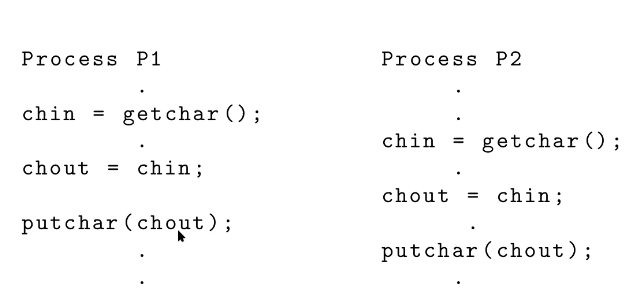
\includegraphics[width=0.5\linewidth]{immagini/ConcorrenzaEsempioChinChoutUnProcessore}
    \caption{Esempio di echo con 2 processi su un processore}
\end{figure}
il problema é dovuto alla concorrenza, perché ci sono piú processi che accedono a memoria condivisa.
\begin{figure}[H]
    \centering
    \includegraphics[width=0.5\linewidth]{immagini/ConcorrenzaEsempioChinChoutPiúProcessori}
    \caption{Esempio di echo con 2 processi su due processori}
\end{figure}
il problema si presenta anche con piú processori, perché chin e chout sono variabili globali, quindi sono in memoria condivisa, quindi anche in questo caso il programma non funziona correttamente.\\
\newline
Per risolvere il problema si puó  pensare che la funzione echo puó essere chiamata da un processo alla volta, o meglio la funzione echo
puó essere chiamata da tanti processi, ma puó essere eseguita da un solo processo alla volta, facendo diventare echo atomica, peró c'é bisogno che qualcuno indichi che
questa funzione é atomica.
\subsection{Race Condition}
Una corsa critica si ha quando piú processi leggono e scrivono una variabile condivisa, e lo fanno in modo tale che il risultato finale dipende dall'ordine in cui vengono eseguiti i processi,
in particolare il risultato puó dipendere dal processo che finisce per ultimo, un sezione critica é la parte di codice di un processo che puó portare ad una corsa critica, nell'esempio 
precedente la sezione critica é l'intera funzione.
\subsection{Per ció che Riguarda il SO}
Il SO deve:
\begin{itemize}
    \item Tenere traccia di vari processi
    \item allocare e deallorare risorse ( CPU, memoria, I/O,file)
    \item Proteggere dati e risorse dall'interferenza (non autorizzata) di altri processi
    \item \textcolor{red}{assicurare che processi ed output siano indipendenti dalla velocitá di computazione (ovvero lo scheduling)}, indipendenti da intendere cum grano salis, rispetto alle specifiche di ciascun processo.
\end{itemize}
\begin{figure}[H]
    \centering
    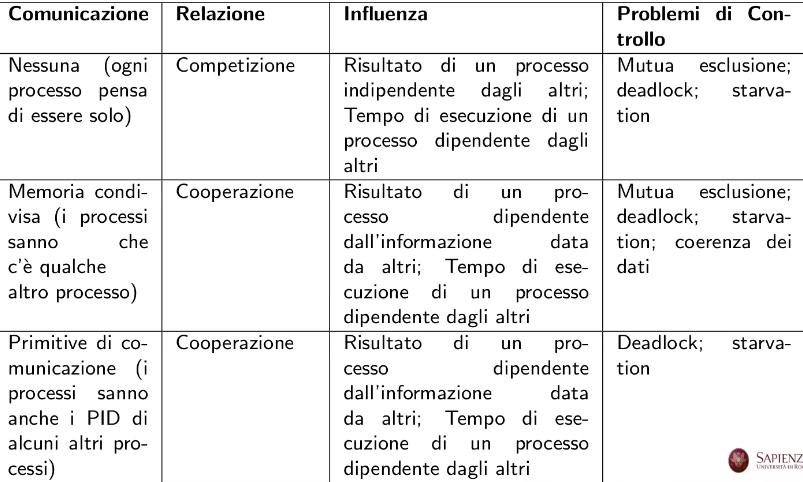
\includegraphics[width=0.7\linewidth]{immagini/RiassuntoComunicazioneTraProcessi}
\end{figure}
\subsection{I processi e la competizione per le risorse}
Il problema é che quando i processi devono accedere ad una risorsa devono chiedere al sistema operativo, quindi la necessitá principale é quella
della mutua esclusione, ovvero solo un processo alla volta puó accedere alla risorsa, peró bisogna stare attenti che comunque non ci siano deadlock e stavation nella systemcall,
\begin{figure}[H]
    \centering
    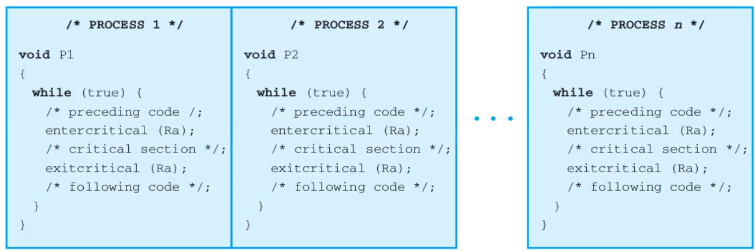
\includegraphics[width=0.7\linewidth]{immagini/MutuaEsclusionePerProcessiInCompetizione}
\end{figure}
Ho una systemcall (Voglio usare il monitor), sostanzialmente la systemcall dovrebbe:
\begin{enumerate}
    \item Entra nella sezione critica (Monitor)
    \item Accede alla risorsa
    \item Esce dalla sezione critica (Fa si che altri processi possano accedere alla risorsa)
\end{enumerate}
questo non é sempre possibile perché potrebbe essere necessario fare una richiesta di blocaggio, quindi ci sono tanti processi che vogliono
accedere alla stessa risorsa, quindi la syscall fa una parte iniziale di controllo per vedere se posso concedere la risorsa, se ci sono
piú processi la syscall deve decidere chi accede alla risorsa, tutti i processi sono visti come dei cicli in cui contiunamente fanno richieste a
determinate risorse.
\subsection{Mutua Esclusione}
\subsubsection*{Mutua Esclusione Processi Cooperanti}
Nei processi cooperanti é il programmatore che si deve occupare della mutua esclusione, il programmatore deve fare in modo che i processi
non accedano contemporaneamente alla stessa risorsa, tutto questo viene fatto tramite strumenti messi a disposizione dal sistema operativo.
\begin{figure}[H]
    \centering
    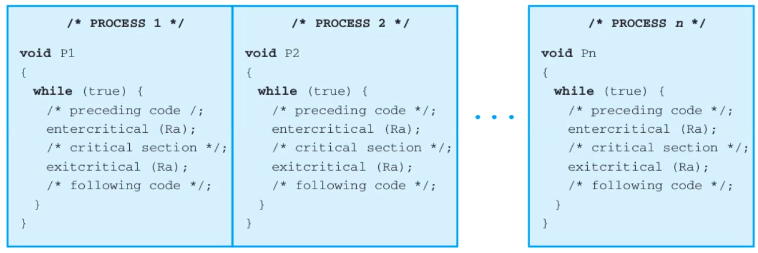
\includegraphics[width=0.7\linewidth]{immagini/MutuaEsclusioneProcessiCooperanti}
\end{figure}
\subsubsection*{Starvation}
Supponiamo che ci siano 2 processi A e B tutti e due richiedono accesso alla stampante, quello che puó
succedere che A rilascia la stampante, ma il sistema operativo lascia A in esecuzione quindi A fa in tempo a
fare un'altra richiesta alla stampante, e quindi il sistema operativo puó decidere di dare la stampante ad A,
in questo modo il processo B puó andare in \textbf{Starvation}
\subsubsection*{Deadlock}
Diciamo che A richiede prima la stampante e poi il monitor, mentre B richiede prima monitor e poi stampante,( \textbf{il fatto che siamo indipendenti dallo scheduler puó essere visto come un diavolo che cerca in tutti i modi di bucare il funzionamento del sistema operativo o delle applicazioni},
quindi dobbiamo fare in modo di metterci nel caso peggiore di scheduling per validare un'applicazione), puó capitare che lo scheduler quindi faccia andare B in mezzo alle 2 richieste di A, quel tanto che basta
per fargli richiedere il monitor, facendo in modo che B prende il monitor e prima che B possa prendere la stampante, faccio tornare A, e quando A
chiede il monitor, il monitor é giá preso da B, e quindi A va in attesa, e quindi B non puó prendere la stampante perché A ha la stampante, e quindi
A e B restano bloccati per sempre, eppure tutto é avvenuto legalmente: la mutua esclusione é stata rispettata, nessuno ha violato la mutua esclusione, peró abbiamo
un deadlock.
\subsubsection*{Requisiti per la mutua esclusione}
\begin{itemize}
    \item Solo un processo alla volta puó essere nella sezione critica per una risorsa
    \item Niente Deadlock e Starvation
    \item Nessuna assunzione su scheduling dei processi, né sul numero dei processi
    \item Un processo deve entrare subito nella sezione critica, se nessun altro processo usa la risorsa (se un solo processo che vuole la risorsa, deve entrare subito)
    \item Un processo che si trova nella sua sezione non-critica non deve bloccare altri processi che richiedono la risorsa (Non puó essere bloccato)
    \item Un processo che sis trova nella sezione critica ne deve prima o poi uscire, piú in general ci vuole cooperazione, Es. non bisogna scrivere un processo che entra nella sua sezione critica senza chiamare entercritical().
\end{itemize}
\subsubsection*{Mutua Esclusione for Dummies}
\begin{lstlisting}[language=C]
    int bolt = 0
    void P(int i)
    {

        while (true)
            bolt = 1;
            while (bolt == 1) /*do nothing*/;
             /* critical section */;

        bolt = 0;
        /* remainder section */;
    }
    parbegin(P(0),P(1),\ldots,P(n-1));
\end{lstlisting}
metto bolt a 1 per prendermi la critical section e aspetto che bolt diventi 0 per uscire dalla critical section, questa é una cosa pessima perché
metto bolt a 1 e non rilascio mai la risorsa per il loop infinito, basta inoltre che lo scheduler faccia eseguire i 2 processi in interleaving perfetto, per avere un deadlock, qundi
va bene la safety, ma ci vuole anche la liveness (almeno un processo ci deve entrare).
\begin{lstlisting}[language=C]
    int bolt = 0
    void P(int i)
    {
        while (true)
            while (bolt == 1) /*do nothing*/;
            bolt = 1;
             /* critical section */;
            bolt = 0;
        /* remainder section */;
    }
    parbegin(P(0),P(1),\ldots,P(n-1));

\end{lstlisting}
quindi facciamo che quando entro nel secondo while, metto bolt a 1, se il dispatcher manda in esecuzione un'altro processo l'altro processo sará in attesa a while (bolt == 1), fino a che
il primo processo non mette bolt a 0, quindi il secondo processo puó entrare nella sezione critica, il problema é che non basta che ci sia qualche scheduling, ma deve essere garantito che
tutti gli scheduling possibili garantiscano l'unicitá di un processo nella sezione critica.
\subsubsection*{Scheduler e Livello Macchina}
Il dispatcher puó interrompere un processo in qualsiasi istante, vuol dire che potrebbe farlo anche prima che un'istruzione sia completata, per esempio nel sedcondo esempio se prendiamo in considerazione
il secondo while del secondo esempio, a livello macchina dobbiamo fare un confronto tra bolt e 1, e sulla base del risultato del confronto, fare un salto oppure andara all'istruzione successiva, supponiamo
che il primo processo P(0) venga eseguito fino a bolt = 1 compreso, si potrebbe pensare che la mutua esclusione sia garantita, ma non é cosí, supponiamo che prima
sia andato in esecuzione P(1), che é riuscito ad arrivare a metá del test di bolt ==1, ovvero carico bolt in un registro e lo confronto con 1, il problema é che
il dispatcher potrebbe aver lasciato caricare il valore di bolt in un registro, poi prima di fare il test manda in esecuzione P(0) che arrivato a bolt = 1, se P(1) riprende
il controllo, il fatto che bolt sia stato messo a 1 da P(0) non lo sa, perché bolt é in memoria, e quindi P(1) potrebbe entrare nella sezione critica, quindi non é garantita la mutua esclusione.
\subsection*{Mutua Esclusione con Interruzioni Disabilitate}
\begin{lstlisting}[language=C]
    while (true)
    {
    /* prima sezione critica */
    disable_interrupts();
    /* sezione critica */
    riabilita_interrupts();
    /* rimanente */
    }
\end{lstlisting}
Una prima soluzione per garantire la mutua esclusione é quella di disabilitare le interruzioni, l'idea quindi é che immediatemnte
prima di entrare nella sezione critica disabilito le interruzioni, in questo modo il dispatcher non puó interrompere il processo, dopo che ho finito la sezione critica
riabilito le interruzioni.
\begin{figure}[H]
    \centering
    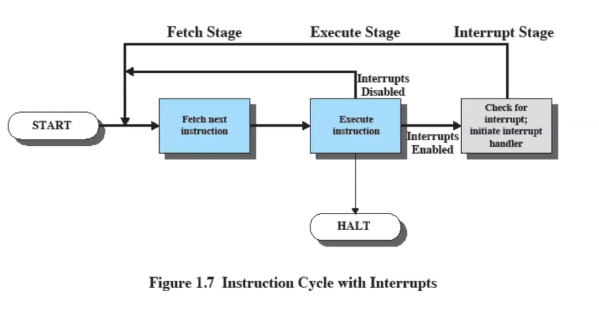
\includegraphics[width=0.5\linewidth]{immagini/DisibilitazioneInterruzzioniMutuaEsclusione}
\end{figure}
Ci sono peró dei problemi, il primo problema é che se do questa possibilitá ai processi utenti é possibile che essi ne
abusino e di conseguenza cala la multiprogrammazzione, inoltre disabilitare le interruzzioni funziona solo se abbiamo un
solo processore, se abbiamo piú processori non funziona, attualmente la disabilitazione delle interruzzioni si fa solo
in kernel mode.
\subsubsection*{Istruzioni speciali macchina}
Esistono delle soluzioni che sono piú accettabili :
\begin{itemize}
    \item \textbf{Compare\_and\_swap}:
    \item \textbf{exchange}
\end{itemize}
L'exchange prende due indirizzi in memoria e scambia i valori, il punto é che sono 3 micro istruzioni, e potrebbe succedere che il processo venga interrotto in qualsiasi punto, ma l'hardware garantisce che se
un processo esegue questa istruzione, nessun altro processo puó eseguire questa istruzione, quindi é garantita la mutua esclusione, e quindi é una istruzione
atomica, quindi é garantita la mutua esclusione.
    \begin{lstlisting}[language=C]{exchange}
        void exchange(int register, int memory)
        {
            int temp
            temp = memory;
            memory = register;
            register = temp;
        }
    \end{lstlisting}
Il compare\_and\_swap é una istruzione che prende 3 parametri, una locazione di memoria, 2 valori, se il valore in memoria é uguale al secondo argomento, allora cambio il valore in memoria con il terzo argomento, in
ogni caso la funzione ritorna il valore vecchio.
\begin{lstlisting}[language=C]{compare_and_swap}
    int compare_and_swap(int word, int testval, int newval)
    {
        int oldval;
        oldval = word;
        if (word == testval)
            word = newval;
        return oldval;
    }
\end{lstlisting}
Subito prima della sezione critica faccio un compare\_and\_swap, che confronta il valore di ritorno della funzione con 1,
al primo processo che arriva cambia il suo valore in 1 e ritorna 0 perché é il vecchio valore, supponiamo che
a questo punto mando in esecuzione un altro processo, esso si troverá con bolt = 1, e quindi non entrerá nella sezione critica, quando il primo processo
esce dalla sezione critica, mette bolt a 0, e quindi il secondo processo puó entrare nella sezione critica.
\begin{figure}[H]
    \centering
    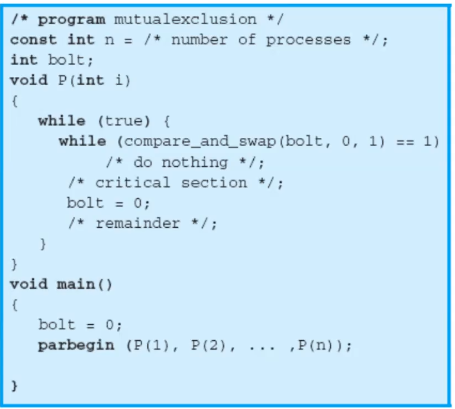
\includegraphics[width=0.7\linewidth]{immagini/CompareAndSwap}
\end{figure}
l'idea é che uso il fatto che bolt sia 1 per i processi successivi al primo per farli stare nel while, quindi non entrano nella sezione critica.\\
\newline
l'exchange si limita a scambiare i valori, per cui l'idea é che ho una variabile locale \textbf{keyi} (ogni processo ha il suo) quindi c'é uno scambio
di valori tra keyi e bolt, se keyi é diverso da 0, allora il processo puó entrare nella sezione critica, altrimenti deve aspettare.
\begin{figure}[H]
    \centering
    \includegraphics[width=0.7\linewidth]{immagini/Exchange}
    \caption{Sbagliato}
\end{figure}
l'errore dietro a questo codice é che il primo che entra va avanti, e rimette bolt a 0, supponiamo che non ci siano altri processi, quando ritorna per un altra richiesta lui si
blocca perché scambia 0 con 0.\\
\newline
I vantaggi di usare queste istruzione sono:
\begin{itemize}
    \item Applicabili a qualsiasi numero di processi, sia su un sistema ad un processore che su un sistema a piú processori
    \item Semplici e quindi facili da verificare
    \item Possono essere usate per gestire sezioni critiche multiple
\end{itemize}
Gli svantaggi sono:
\begin{itemize}
    \item Sono basati sul concetto di busy-waiting, il punto é che queste soluzioni devono continuamente ciclare fino a che non possono entrare nella sezione critica, dal punto di vista del sistema operativo lui non ha modo di distinguere un processo che sta facendo una istruzione speciale da una che sta facendo un'altro tipo di operazioni, quindi dal punto di vista del dispatcher questi processi sono ready e non possono essere esclusi, questa cosa é inevitabile, se siamo in un sistema operativo con dispatcher round robin viene eseguito fino a time-out
    \item Possibile Starvation: supponiamo 2 processi P(1) passa, va in esecuzione P(2) dopo di che il dispatcher da la CPU a P(1) che va in esecuzione, e potrebbe riuscire a rientrare di nuovo nella sezione critica, e quindi P(2) va in starvation
    \item Possibile Deadlock: se abbiamo una prioritá fissa tra i processi, es. P(1) con prioritá bassa e P(2) con prioritá alta, P(1) esce dalla sezione critica e P(2) entra, se P(1) rientra nella sezione critica, P(2) entra in sezione critica e P(1) non riesce piú ad entrare.
\end{itemize}
\subsection{Semafori}
In molti caso per evitare il busy waiting si possono usare i semafori,che sono delle particolari strutture dati sulle quali é
possibile fare 3 operazioni \textbf{Atomiche} garantite dal sistema operativo:
\begin{itemize}
    \item Initialize
    \item decrement o semWait : puó mettere il processo in blocked per cui niente CPU sprecata come con il busy waiting
    \item increment o semSignal : puó mettere un processo blocked in ready
\end{itemize}
I semafori racchiudono al loro interno un contatore, che puó essere decrementato o incrementato, la cosa interessante é che l'operazione di decremento che viene chiamata wait
puó mettere in blocked il processo che la chiama, questo evita quindi il busy waiting, per contro l'operazione di incremento puó mettere in ready un processo che era blocked,
stiamo quindi considerando un'altro tipo di blocked rispetto a quello che abbiamo visto con l'I/O, in questo caso il processo é blocked perché é in attesa di un semaforo,
ovviamente essendo syscall, sono istruzioni che vengono eseguite in kernel mode e possono agire direttamente sui processi.
\begin{figure}[H]
    \centering
    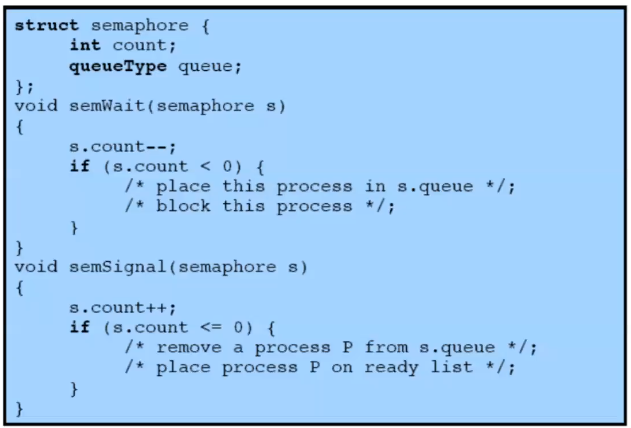
\includegraphics[width=0.7\linewidth]{immagini/ImplementazioneSemaforo}
\end{figure}
un semaforo quindi é composto da un intero e da una coda di processi, se facciamo una wait significa che decremento il contatore,
se come risultato il contatore é negativo allora il processo che ha fatto questa chiamata va bloccato e messo in coda, invece una
signal incrementa di 1 il contatore, se il valore é ancora negativo, significa che c'é qualcosa da sbloccare, per cui dalla coda
vado a scegliere uno dei processi, lo tolgo e lo metto in ready.
\begin{figure}[H]
    \centering
    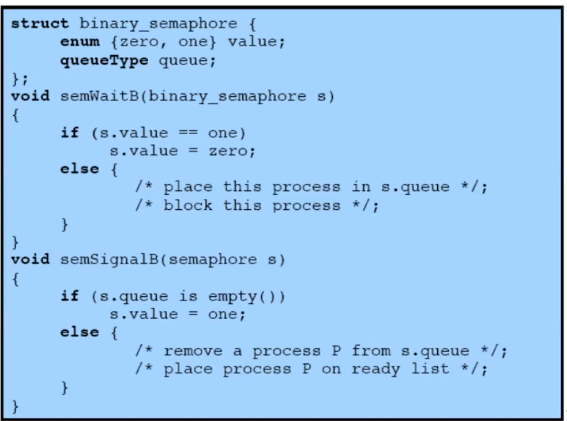
\includegraphics[width=0.7\linewidth]{immagini/ImplementazioneSemaforiBinari}
\end{figure}
In un semaforo binario il valore non é piú un intero, ma un booleano, quindi il valore puó essere 0 o 1, l'idea
peró rimane la stessa, se il valore é 0 il processo va in blocked, se la coda é vuota allora metto il valore a 1,
invece se ci sono processi in coda, prendo uno di questi processi e lo metto in ready.
\begin{figure}[H]
    \centering
    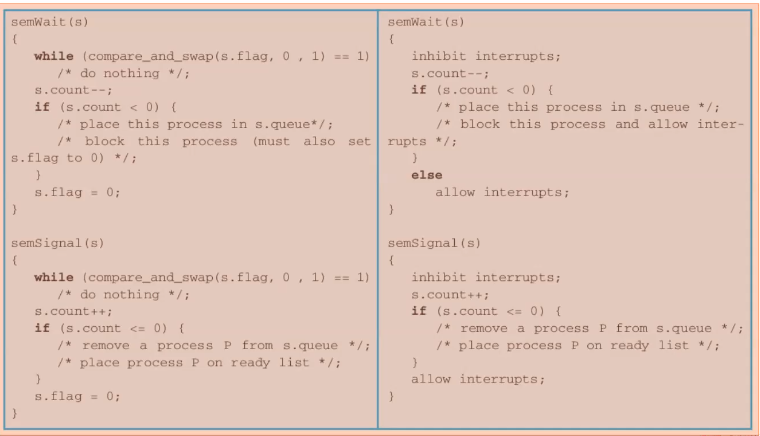
\includegraphics[width=0.7\linewidth]{immagini/PossibileImplementazioneDiSemafori}
\end{figure}
In questa maniera il busy waiting viene ridotto al minimo, se sono su un solo processore, disabilito le interruzzioni.
\subsubsection{semafori Deboli e Forti}
Si parla di semafori deboli e di semafori forti, a seconda di come devo scegliere il processo da sbloocare, i semafori forti sono quelli
che usano una coda FIFO, se la politica non viene specificata, allora si parla di weak semaphore, sappiamo quindi che un generico processo
viene sbloccato, con i semafori forti, é possibile inoltre evitare la starvation.
\begin{figure}[H]
    \centering
    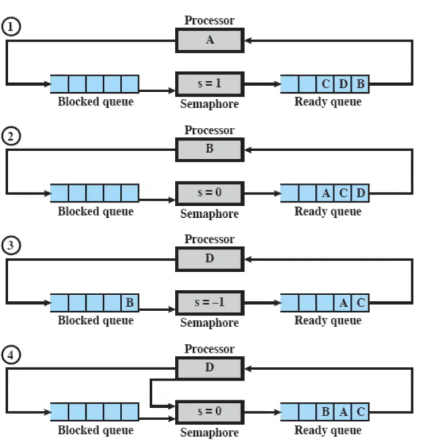
\includegraphics[width=0.7\linewidth]{immagini/SemaforiForti}
\end{figure}
\begin{enumerate}
    \item Faccio una wait, il contatore va a 0 , ma il processo no va blocked perché il contatore é maggiore di 0
    \item Faccio un'altra wait, il contatore va a -1, il processo va in blocked e va in esecuzione
    \item D fa signal, il contatore va a 0, il processo B ritorna nella coda dei ready
\end{enumerate}
\begin{figure}[H]
    \centering
    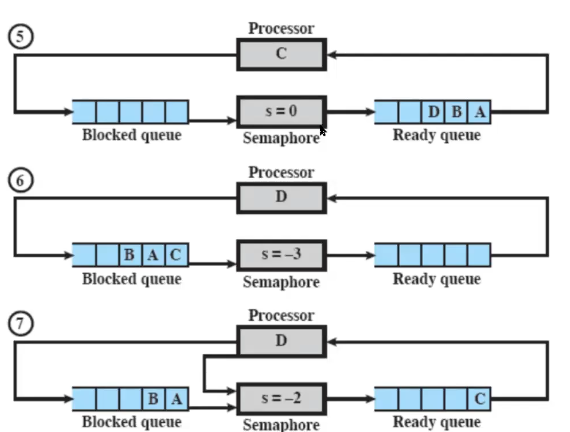
\includegraphics[width=0.7\linewidth]{immagini/SemaforiForti2}
\end{figure}
In questa seconda parte faccio 3 wait e mando in blocked i tre processi, poi faccio 3 signal, ed in ordine FIFO sblocco i
processi in blocked.
\begin{figure}[H]
    \centering
    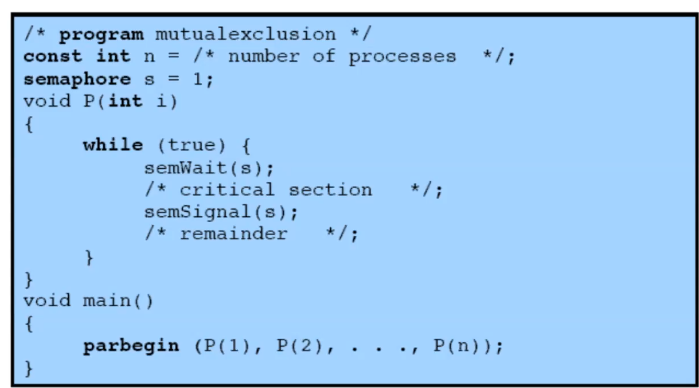
\includegraphics[width=0.7\linewidth]{immagini/MutuaEsclusioneConSemafori}
\end{figure}
A questo punto non c'é starvation,se siamo tra due processi non c'é in nessun caso, con piú di due processi
ci potrebbe essere solo con i semafori deboli, perché potrebbe succedere di sbloccare solo alcuni processi.
\begin{figure}[H]
    \centering
    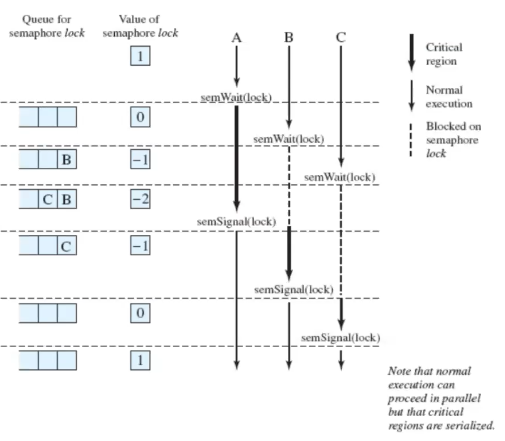
\includegraphics[width=0.7\linewidth]{immagini/EsecuzioneSemafori}
\end{figure}
\subsection{Produttore-Consumatore}
Ci sono casi in cui siamo interessati ad avere processi che cooperano per risolvere un problema, un esempio é quello del produttore-consumatore,
La situazione é la seguente:
\begin{itemize}
    \item Un processo produttore che crea dati e li mette in un buffer
    \item Un consumatore che legge i dati dal buffer creati dal consumatore
    \item al buffer puó accedere un solo processo alla volta
\end{itemize}
Il problema é quello di garantire la mutua esclusione nell'accesso, ma il vero problema che voglio risolvere é assicurare che
i produttori non inseriscano i dati se il buffer é pieno, ed il consumatore non deve prendere dati se il buffer é vuoto, il progettista
deve fare in modo che il produttore aspetti se il buffer é pieno, e il consumatore aspetti se il buffer é vuoto, in realtá ci sono molte
varianti di questo problema, essenzialmente potremmo vedere il buffer come una coda, e quindi il produttore mette i dati in coda e il consumatore
li toglie dalla coda, ma noi considereremo il buffer come una entitá ad accedere in mutua esclusione, supponiamo inizialmente che il buffer
sia infinito allora:
\begin{lstlisting}[language=C]
    while (true){
    /* produce an item v*/
    b[in] = v;
    in++;
    }
\end{lstlisting}
\begin{lstlisting}[language=C]
    while (true){
        while (in <= out) /* do nothing  in attesa che out sia piú piccolo di in*/;
        w = b[out];
        out++;
        /* consume the item w */
    }
\end{lstlisting}
Da notare che la fase di produzione e di consumo sono da considerare operazioni locali quindi non c'é nessun problema se
il produttore e il consumatore fanno queste operazioni in parallelo, v e w sono variabili locali, e almeno in deve essere globale.
\begin{figure}[H]
    \centering
    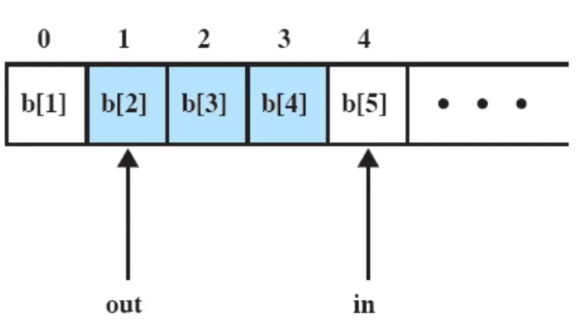
\includegraphics[width=0.7\linewidth]{immagini/ProduttoreConsumatoreBuffer}
\end{figure}
\subsubsection*{Soluzione al Problema}
\begin{figure}{H}
    \centering
    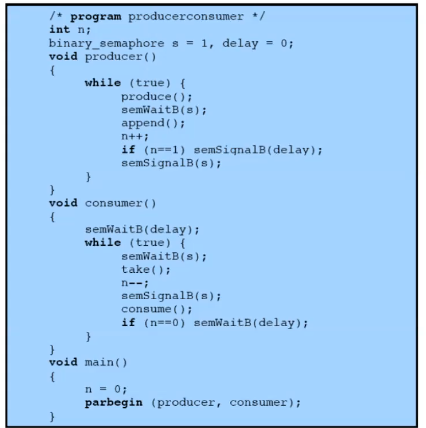
\includegraphics[width=0.7\linewidth]{immagini/ProduttoreConsumatoreSoluzioneSbagliata}
    \caption{Sbagliata}
\end{figure}
Una prima implementazione che potremmo pensare é quella riportata nell'immagine sopra che usa i
semafori binari, nel nostro caso s=1 e delay =0, abbiamo un main con 2 processi, il produttore e il consumatore, essenzialmente c'é un controllo che
ci sia la mutua esclusione sul buffer, questa cosa é controllata dal semaforo s, non deve succedere quindi che il consumatore cerchi di consumare
con la coda vuota, oltre ai 2 semafori abbiamo una variabile condivisa n intera, durante la produzione incremento n , durante il consumo decremento n,
quindi n rappresenta il numero di elementi nel buffer, l'idea é che il consumatore che va in esecuzione per primo si blocca perché delay é 0,
quindi é necessario che il produttore vada in esecuzione per primo, a questo punto il produttore mette a 1 il semaforo delay, sbloccando quindi
la possibilitá che il consumatore possa andare in esecuzione, l'idea é \textbf{ho messo un nuovo elemento dopo che il buffere é vuoto allora sblocco il consumatore},
se dopo che ho consumato n diventa 0 allora mi devo bloccare, sembra sia una soluzione corrette, ma non lo é , infatti potrebbe succedere che a metá tra
tra il consume ed il controllo che n sia = 0, il produttore mette un nuovo elemento, e quindi il consumatore non si blocca, essenzialmente per risolvere il problema dopo il decremento di
n mi salvo il suo valore in una variabile locale, e quindi se viene richiamato il produttore che modifica n, io mi ricordo il vecchio valore di n.
\begin{figure}[H]
    \centering
    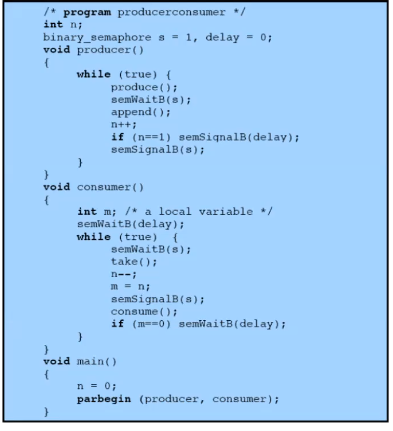
\includegraphics[width=0.7\linewidth]{immagini/SoluzioneProduttoreConsumatoreCorretta}
\end{figure}
\begin{figure}[H]
    \centering
    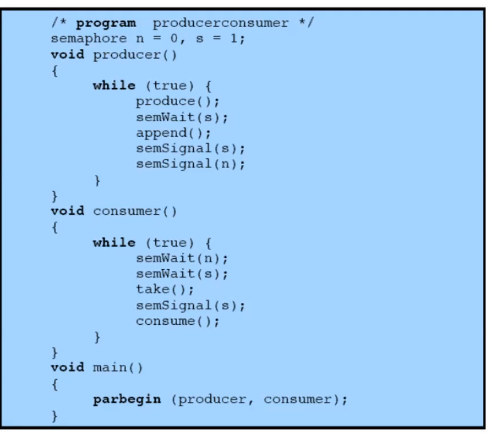
\includegraphics[width=0.7\linewidth]{immagini/SoluzioneProduttoreConSemaforiGenerali}
\end{figure}
Qualsiasi cosa scritta con semafori binari si puó scrivere con semafori generali, vale anche il viceversa.
\subsection{Produttore consumatore con buffer circolare}
\begin{figure}[H]
    \centering
    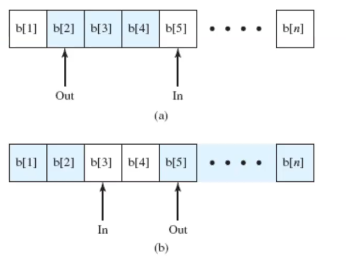
\includegraphics[width=0.7\linewidth]{immagini/ProduttoreConsumatoreBufferCircolare}
\end{figure}
Mettiamoci quindi nel caso in cui il buffer sia finito, quindi c'é una regione finita di memoria, che é dedicata al buffer,
ed é gestita in maniera circolare, perché non si possono fare assunzioni su quanto sia veloce il produttore e il consumatore,
potrebbe succedere che il dispatcher dia tempo al produttore di produrre 10 elementi, e il consumatore ne consumi 5, quindi
questo si realizza con un buffer circolare, nell'immagine ci sono n slot nel buffer dove si possono mettere gli oggetti da consumare,
l'idea é che esistono 2 puntatori in e out, in é il puntatore che indica dove mettere il prossimo elemento, out é il puntatore che
indica dove prendere il prossimo elemento,c'é un problema, che é dovuto al fatto che se in e out sono uguali, il buffer puó essere sia pieno
che vuoto, se lo pensiamo in maniera circolare, se per esempio: se n=5 , ed il consumatore non fa niente, ed il produttore mette 5 elementi,
nel buffer se partivamo da uno stato vuoto, in = 0 e out = 0, dopo che il produttore ha messo 5 elementi, in = 0 e out = 0, quindi in e out sono uguali,
ma il buffer é pieno, per questo motivo dobbiamo sacrificare uno slot, quindi il buffer avrá n-1 slot, a questo punto in=out significa che il buffer é vuoto,
invece é pieno se $in + 1 mod (buffer) = out$, con questo scenario le cose rimangono simili a prima, addesso c'é un controllo sul pieno e sul vuoto.
\begin{lstlisting}[language=C]
    /*produce an item v */
    while (true){
        while ((in + 1) % n == out) /* do nothing */;
        b[in] = v;
        in = (in + 1) % n;
    }
\end{lstlisting}
\begin{lstlisting}[language=C]

    while (true){
        while (in == out) /* do nothing */;
        v = b[out];
        out = (out + 1) % n;
        /* consume the item w */
    }
\end{lstlisting}

come facciamo quindi a scrivere una funzione con i semafori per risolvere il problema del produttore consumatore con buffer circolare? La soluzione
di prima chiaramente non funzionerebbe perché non c'é un controllo sul pieno e sul vuoto, per risolverlo quindi abbiamo bisogno di un terzo semaforo.

\begin{figure}[H]
    \centering
    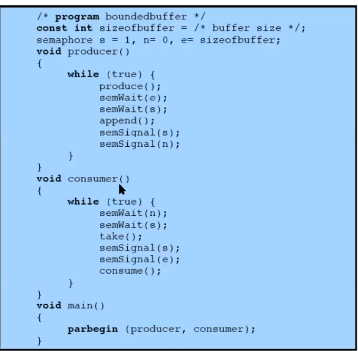
\includegraphics[width=0.7\linewidth]{immagini/ProduttoreConsumatoreConBufferCircolare}
\end{figure}
quindi partiamo con un terzo semaforo inizializzato alla lunghezza del buffer, il trucco é
\begin{enumerate}
    \item Nel consumatore faccio subito una semWait su n cosí se sono il primo mi blocco
    \item Nel produttore faccio subito una semWait su e, cosí se sono da solo e faccio subito sizeOfBuffer iterazioni, mi blocco.
    \item ad ogni Wait deve corrispondere una signal, in modo che il produttore possa svegliare il consumatore e viceversa.
\end{enumerate}
questa é la soluzione classica di \textbf{Un produttore e un consumatore}.
\subsection{Mutua Esclusione: Soluzioni software}
Fino adesso abbiamo fatto riferimento a soluzioni atomiche, diamo uno sguardo a soluzioni, per risolvere
problemi di mutua esclusione, che non sono atomiche, ovvero che non sono garantite dal sistema operativo.

Esempio ci sono due processi che vogliono fare la critical section uno per volta, cerchiamo di capire come
possiamo garantire questa cosa, facendo solo assegnamento a variabili, facciamo un primo tentativo (questa cosa funziona solo per 2 processi),
\begin{figure}[H]
    \centering
    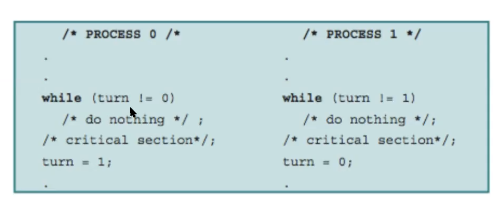
\includegraphics[width=0.7\linewidth]{immagini/MutuaEsclusionePrimoTentativo}
\end{figure}
Una prima soluzione potrebbe essere che ho una variabile condivisa tra i due processi, se turn é 0 P(0) si blocca,
se turn é 1 P(1) si blocca, chiaramente adesso é tutta attesa attiva, é chiaro che una soluzione come questa risolve il
problema della mutua esclusione,se un processo é da solo e vuole accedere alla sezione critica non lo puó fare.

\begin{figure}[H]
    \centering
    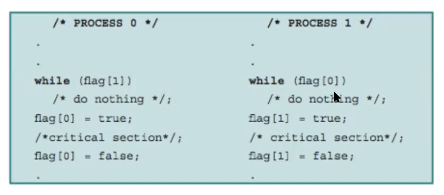
\includegraphics[width=0.7\linewidth]{immagini/MutuaEsclusioneSecondoTentativo}
\end{figure}
Invece che usare turn, uso un vettore (2 variabilli globali), il processo 0 legge la variabile dell'altro e modifica
la propia, il processo 1 fa la stessa cosa, ovviamente questo non puó andare bene, se entrambi sono a 0 potrebbe succedere
che entrambi entrano nella sezione critica, quindi non é garantita la mutua esclusione.

\begin{figure}[H]
    \centering
    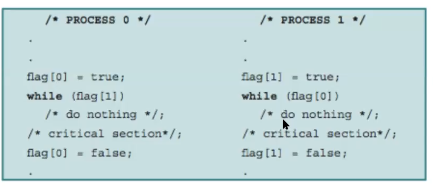
\includegraphics[width=0.7\linewidth]{immagini/MutuaEsclusioneTerzoTentativo}
\end{figure}

Metto il flag a 1, ad entrambi i processi, e poi faccio un while, il flag indica l'intento di iniziare
la sezione critica, peró se faccio di nuovo un interleave perfetto, potrebbe succedere che entrambi i processi
entrino in deadlock

\begin{figure}[H]
    \centering
    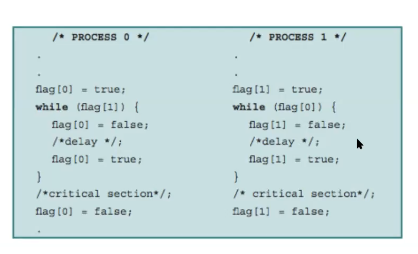
\includegraphics[width=0.7\linewidth]{immagini/MutuaEsclusioneQuartoTentativo}
\end{figure}

Invece di non fare niente provo, a dichiararmi inizialmente come non interessato a entrare nella sezione critica, e poi
metto il flag a 0, e dopo un delay metto il flag a 1, mentre sono in attesa, l'idea é che se introduco un ritardo
random, allora con una buona probabilitá succede che il processo uno fa in tempo a mettere il suo flag a true, ma
il processo 0 non riesce a mettere a true il suo flag, quindi il processo 1 entra nella sezione critica, potrebbe effettivamente
funzionare in un discorso con alta probabilitá, peró non é garantito, quindi non é una soluzione corretta.
\subsubsection*{Algoritmo Di Dekker}
\begin{figure}[H]
    \centering
    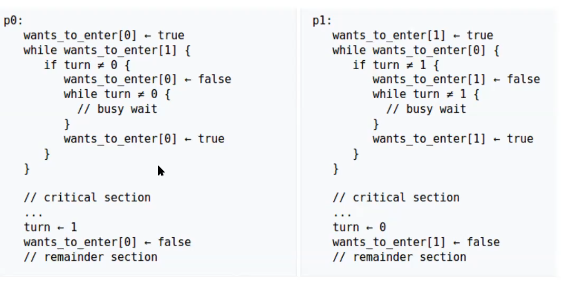
\includegraphics[width=0.7\linewidth]{immagini/Dekker}
\end{figure}
Solo una variabile condivisa non basta, solo 2 varibaili booleane non bastano, proviamo quindi a mettere insieme
le due idee, succede che fin dall'inizio dichiaro di voler provare ad entrare nella sezione critica, l'idea é che c'é
una variabile turn condivisa, se per caso non tocca a me rimetto a falso il fatto che voglio entrare e faccio una
attesa attiva, fino a che turn continua ad essere l'altro, quando esco rimetto wants to enter a true, si puó dimostrare
matematicamente che questa soluzione funziona.

Questa soluzione vale solo per 2 processi, se ci sono piú processi, non é cosí semplice, garantisce la non starvation,
garantisce che non ci siano deadlock e non richiede nessun supporto dal sistema operativo e dall'hardware, ci sono alcune
architetture che potrebberó riordinare le istruzioni, chiaramente se ció succede l'algoritmo non funziona piú.

\subsubsection*{Algoritmo Di Peterson}
\begin{figure}[H]
    \centering
    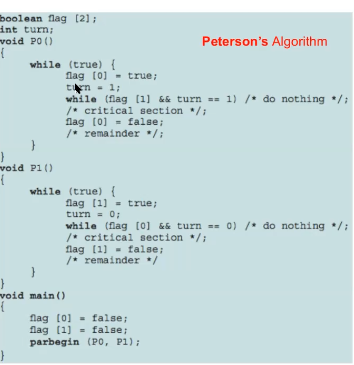
\includegraphics[width=0.7\linewidth]{immagini/AlgoritmoDIPeterson}
\end{figure}
Anche qui il processo che vuole entrare segnala che vuole entrare, per quanto riguarda la variabile turn, viene acceduto in
scrittura prima della critical section, il processo 0 dice di passare al processo 1 e viceversa, in questa maniera
anche se facessimo un interleave perfetto, o P0 setta turn 1 o P1 setta turn 0, l'ultimo che fa l'assegnamento vince, alla fine
l'unica cosa che serve dopo la critical section bisogna mettere a 0 il proprio flag.

Questa soluzione vale solo per 2 processi, anche se é piú semplice estenderlo ad N processi, é possibile la bounded waiting.

\subsection{Comunicazione Esplicita}

É possibile che un processo mandi un messaggio ad un altro processo, per fare message passing funziona sia con memoria condivisa
che distribuita, puó essere anche usata per la sincronizzazione, le funzionalita di message passing sono:
\begin{itemize}
    \item send (destinatario, messaggio da inviare)
    \item receive (mittente, messaggio (zona di memoria dove voglio mettere i valori))
    \item spesso c'é anche un test di ricezioine
    \item notare che message é un input per la send ed un output per la receive
\end{itemize}
\subsubsection{Sincronizzazione}
La comunicazione richiede anche una sincronizzazione, tra i processi, allora prima il mittente deve inviare e poi il ricevente deve ricevere,
queste operazioni possono essere bloccanti ed operazioni che non bloccano, il test di ricezione non é mai bloccante.
\subsubsection*{Send e receive bloccanti}
Il processo che fa la send si blocca fino a che il processo che fa la receive non riceve il messaggio, quando il processo riceve il messaggio allora
si sblocca il processo che ha fatto la send, tipicamente questo tipo di comunicazione si chiama randez-vous.
\subsubsection*{Send non bloccante}
Con ricezione bloccante, il mittente continua (non si blocca) il destinatario rimane bloccato finché non ha ricevuto il messaggio,
Con ricezione non bloccante, se il messaggio c'é viene ricevuto, altrimenti il destinatario continua, la receive non bloccante puó settare un bit dentro il messaggio
per dire se la ricezione é avvenuta oppure no, se la ricezione non é bloccante anche il mittente non é bloccante, sono operazioni atomiche, un solo processo per volta le esegue ed
finché l'operazione non é completata, oppure il processo non viene bloccato.
\subsection{Indirizzamento}
Il mittente deve poter dire a quale processo mandare il messaggio(o quali processi), lo stesso vale per il destinatario, ci sono 2 modi per fare l'indirizzamento:
\begin{itemize}
    \item Diretto: il mittente sa l'identitá del destinatario
    \item Indiretto: il mittente sa l'identitá di un intermediario che sa l'identitá del destinatario.
\end{itemize}
\subsubsection*{Indirizzamento Diretto}
Nell'indirizzamento diretto la send ha come parametro il destinatario, per la receive invece puó essere presente oppure no es:
\begin{lstlisting}[language=C]
    send(destinatario, messaggio);
    receive(mittente, messaggio);
\end{lstlisting}
oppure
\begin{lstlisting}[language=C]
    send(destinatario, messaggio);
    receive(null,messaggio);
\end{lstlisting}
questo succede perché dentro al messaggio é presente anche il mittente, inoltre ogni processo ha una sua coda per i messaggi; una volta piena, solitamente il messaggio si perde o
viene ritrasmesso.
\subsubsection*{Indirizzamento Indiretto}
Nell'indirizzamento indiretto i messaggi vengono mandati ad una mailbox (Zona di memoria condivisa) ed va esplicitamente creata,il mittente manda messaggi alla mailbox,
da dove il destinatario li prende, \textcolor{red}{se la ricezione é bloccante e ci sono piú processi in attesa su una ricezione, un solo processo viene sbloccato}
Ci sono quindi evidenti analogie con il problema del produttore/consumatore, in particolare, se la mailbox é piena allora anche nbsend si deve bloccare, se serve solo per le
versioni bloccanti, e per comunicazioni x-to-one, la mailbox puó avere dimensione 1.
\begin{figure}[H]
    \centering
    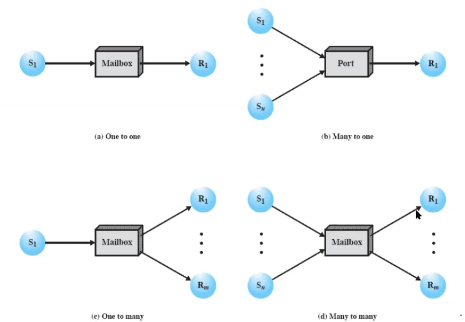
\includegraphics[width=0.7\linewidth]{immagini/ComunicazioneIndiretta}
\end{figure}
\subsection{Struttura dei messaggi}
\begin{figure}[H]
    \centering
    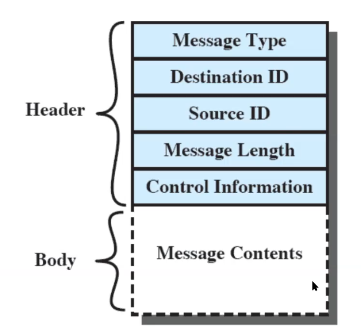
\includegraphics[width=0.7\linewidth]{immagini/StrutturaDiUnMessaggio}
\end{figure}
Di solito quando intendiamo un messaggio quello che intendiamo é il contenuto del messaggio(BODY), ma in realtá un messaggio é composto da:
\begin{itemize}
    \item \textbf{Header}: contiene informazioni sul messaggio, come il mittente, il destinatario, la lunghezza del messaggio, il tipo di messaggio, control information.
    \item \textbf{Body}: contiene il contenuto del messaggio
\end{itemize}
le informazioni che si trovano nell'header sono chiamate meta-dati.
\subsection{Usare i messaggi per risolvere la mutua esclusione}
\begin{lstlisting}[language=C]
    const messagge null = /* null message */;
    mailbox box;
    void P(int i) {
        message m;
        while (true){
            receive(box, m);
            /* sezione critica */
            nbsend(box, m);
            /* resto */
        }
    }
    void main() {
        box = create_mailbox();
        nb_send(box, null);
        parbegin(P(0), P(1));
    }
\end{lstlisting}
Se io eseguo P senza inizializzazione non funzione, perché qualsiasi processo arriva si blocca sulla receive, questo
funziona perché c'é la parte di inizializzazione nel main, prima di mandare gli n processi inizializzo la mailbox con un messaggio nullo,
e mando in esecuzione i processi, se anche uno di questi processi arriva a ricevere il messaggio allora esegue la critical section, per poi
rilasciare con un nbsend, se la send nel main la send é bloccante avremmo un problema perché i processi non andrebbero in esecuzione, invece
all'interno di P potrei metterla bloccante, peró non é efficiente
\subsection{Producer-Consumer con Message Passing}
\begin{lstlisting}[languace = C]
    const int capacity = /* dimensione del buffer */;
    mailbox mayproduce, mayconsume;
    const message null = /* null message */;
    void main(){
        mayproduce = create_mailbox();
        mayconsume = create_mailbox();
        for (int i = 1; i <= capacity; i++)
            nb_send(mayproduce, null);
        parbegin(producer(), consumer());
    }
\end{lstlisting}
\begin{lstlisting}[language = C]
    void producer(){
        message m;
        while (true){
            receive(mayproduce, m);
            /* produce an item */
            nbsend(mayconsume, m);
        }
    }
\end{lstlisting}
\begin{lstlisting}[language = C]
    void consumer(){
        message m;
        while (true){
            receive(mayconsume, m);
            /* consume an item */
            nbsend(mayproduce, m);
        }
    }
\end{lstlisting}
All'inizion mayconsume é vuota quindi il consumatore si blocca se va in esecuzione per primo, quindi il produttore puó produrre e riempire mayconsume.























































